\documentclass[12pt, letterpaper]{article}
\pagestyle{empty}

\usepackage[utf8]{inputenc}
\usepackage{amsmath, amssymb} \allowdisplaybreaks
\usepackage{xcolor}
\usepackage{graphicx}
\usepackage{tikz}
\usepackage[margin=1in]{geometry}
\usepackage{indentfirst}
\usepackage{multicol}

\begin{document}
\definecolor{myColor}{HTML}{03468F}
\color{myColor}

    \section{Which of the relations above do not represent functions? Justify your answer.}

        \subsection{Relation \(R_2\) }
        \vspace{-18pt}
        \begin{align*}
            & R_2 \; = \; \Bigl\{ (1, 2), (2, 2), (3, 3), (4, 4), (2, 3), (5, 2) \Bigr\} \\
            & \implies \Big(\big(2, 2\big) \in R_2\Big) \wedge \Big(\big(2, 3\big) \in R_2\Big) \\ 
            & \implies \exists x \exists y_1 \exists y_2 \; \Big( \big(x, y_1\big) \in R_2 \Big) \wedge
                                                   \Big( \big(x, y_2\big) \in R_2 \Big) \wedge
                                                   \Big( y_1 \neq y_2 \Big) \\
            & \implies \exists x \exists y_1 \exists y_2 \; \Big( \big(x, y_1\big) \in R_2 \Big) \wedge
                                                   \Big( \big(x, y_2\big) \in R_2 \Big) \wedge
                                                   \neg\Big( y_1 = y_2 \Big) \\
            & \implies \exists x \exists y_1 \exists y_2 \; \Big( \big(x, y_1\big) \in R_2 \wedge
                                                   \big(x, y_2\big) \in R_2 \Big) \wedge
                                                   \neg\Big( y_1 = y_2 \Big) \\
            & \implies \exists x \exists y_1 \exists y_2 \; \neg\Big( \big(x, y_1\big) \in R_2 \wedge
                                                   \big(x, y_2\big) \in R_2 \Big) \lor
                                                   \Big( y_1 = y_2 \Big) \\
            & \implies \exists x \exists y_1 \exists y_2 \; \Big( \big(x, y_1\big) \in R_2 \wedge
                                                   \big(x, y_2\big) \in R_2 \Big) \implies
                                                   \Big( y_1 = y_2 \Big) \\
            & \implies \neg\forall x \forall y_1 \forall y_2 \; \Big( \big(x, y_1\big) \in R_2 \wedge
                                                   \big(x, y_2\big) \in R_2 \Big) \implies
                                                   \Big( y_1 = y_2 \Big) \\
            & \implies \neg\Big( R_2 : D_{R_2} \to R_{R_2} \Big)
              \implies \text{ \(R_2\) is not a function.}
        \end{align*}

        \subsection{Relation \(Q\)}
        \vspace{8pt}
        \begin{center}
            \begin{tikzpicture}[>=stealth, node distance=2cm, baseline={(current bounding box.center)}]
                \node (label) at (0,1.233) {\(Q \qquad = \quad\)};

                \node (a) at (2,2) {$a$};
                \node (b) at (2,1.5) {$b$};
                \node (c) at (2,1) {$c$};

                \node (1) at (4,2) {$1$};
                \node (2) at (4,1.5) {$2$};
                \node (3) at (4,1) {$3$};
                \node (4) at (4,0.5) {$4$};

                \draw[->] (a) -- (1);
                \draw[->] (b) -- (2);
                \draw[->] (c) -- (3);
                \draw[->] (c) -- (4);
            \end{tikzpicture}
        \end{center}
        \begin{align*}
            & \implies \Big(\big(c, 3\big) \in Q\Big) \wedge \Big(\big(c, 4\big) \in Q\Big) \\ 
            & \implies \exists x \exists y_1 \exists y_2 \; \Big( \big(x, y_1\big) \in Q \Big) \wedge
                                                   \Big( \big(x, y_2\big) \in Q \Big) \wedge
                                                   \Big( y_1 \neq y_2 \Big) \\
            & \implies \exists x \exists y_1 \exists y_2 \; \Big( \big(x, y_1\big) \in Q \Big) \wedge
                                                   \Big( \big(x, y_2\big) \in Q \Big) \wedge
                                                   \neg\Big( y_1 = y_2 \Big) \\
            & \implies \exists x \exists y_1 \exists y_2 \; \Big( \big(x, y_1\big) \in Q \wedge
                                                   \big(x, y_2\big) \in Q \Big) \wedge
                                                   \neg\Big( y_1 = y_2 \Big) \\
            & \implies \exists x \exists y_1 \exists y_2 \; \neg\Big( \big(x, y_1\big) \in Q \wedge
                                                   \big(x, y_2\big) \in Q \Big) \lor
                                                   \Big( y_1 = y_2 \Big) \\
            & \implies \exists x \exists y_1 \exists y_2 \; \Big( \big(x, y_1\big) \in Q \wedge
                                                   \big(x, y_2\big) \in Q \Big) \implies
                                                   \Big( y_1 = y_2 \Big) \\
            & \implies \neg\forall x \forall y_1 \forall y_2 \; \Big( \big(x, y_1\big) \in Q \wedge
                                                   \big(x, y_2\big) \in Q \Big) \implies
                                                   \Big( y_1 = y_2 \Big) \\
            & \implies \neg\Big( Q : D_{Q} \to R_{Q} \Big)
              \implies \text{ \(Q\) is not a function.}
        \end{align*}

        \subsection{Relation \(r\) }
        \begin{center}
            \includegraphics[width=0.3\textwidth]{relation_r.png}
        \end{center}
        \begin{align*}
            & \implies \Big(\big(2, 3\big) \in r\Big) \wedge \Big(\big(2, 4\big) \in r\Big) \\ 
            & \implies \exists x \exists y_1 \exists y_2 \; \Big( \big(x, y_1\big) \in r \Big) \wedge
                                                   \Big( \big(x, y_2\big) \in r \Big) \wedge
                                                   \Big( y_1 \neq y_2 \Big) \\
            & \implies \exists x \exists y_1 \exists y_2 \; \Big( \big(x, y_1\big) \in r \Big) \wedge
                                                   \Big( \big(x, y_2\big) \in r \Big) \wedge
                                                   \neg\Big( y_1 = y_2 \Big) \\
            & \implies \exists x \exists y_1 \exists y_2 \; \Big( \big(x, y_1\big) \in r \wedge
                                                   \big(x, y_2\big) \in r \Big) \wedge
                                                   \neg\Big( y_1 = y_2 \Big) \\
            & \implies \exists x \exists y_1 \exists y_2 \; \neg\Big( \big(x, y_1\big) \in r \wedge
                                                   \big(x, y_2\big) \in r \Big) \lor
                                                   \Big( y_1 = y_2 \Big) \\
            & \implies \exists x \exists y_1 \exists y_2 \; \Big( \big(x, y_1\big) \in r \wedge
                                                   \big(x, y_2\big) \in r \Big) \implies
                                                   \Big( y_1 = y_2 \Big) \\
            & \implies \neg\forall x \forall y_1 \forall y_2 \; \Big( \big(x, y_1\big) \in r \wedge
                                                   \big(x, y_2\big) \in r \Big) \implies
                                                   \Big( y_1 = y_2 \Big) \\
            & \implies \neg\Big( r : D_{r} \to R_{r} \Big)
              \implies \text{ \(r\) is not a function.}
        \end{align*}


    \newpage
    \section{Assume that each of the functions listed above is onto. Find the domain and range of each function.}

        \subsection{Function \(R_1\)}
        \vspace{-2pt}
        \begin{minipage}{0.5\textwidth}
            \begin{align*}
                & D_{R_1} = \{a, b, c, m\}
            \end{align*}
        \end{minipage}
        \begin{minipage}{0.5\textwidth}
            \begin{align*}
                & R_{R_1} = \{1, 2, 3, 5\}
            \end{align*}
        \end{minipage}
        
        \subsection{Function \(I\)}
        \vspace{-2pt}
        \begin{minipage}{0.5\textwidth}
            \begin{align*}
                I(x) &= x^2 - 1 \\
                D_{I} &= \mathbb{R}
            \end{align*}
        \end{minipage}
        \begin{minipage}{0.5\textwidth}
            \begin{align*}
                I(x) &= x^2 - 1 \\
                x^2 &= I(x) + 1 \\
                x &= \pm\sqrt{I(x) + 1} \\
                I(x) + 1 &\geq 0 \\
                I(x) &\geq -1 \\
                R_{I} &= \left[-1, \infty\right)
            \end{align*}
        \end{minipage}

        \subsection{Function \(J\)}
        \vspace{-2pt}
        \begin{minipage}{0.5\textwidth}
            \begin{align*}
                J(x) &= 2x + 3 \\
                D_{J} &= \mathbb{R}
            \end{align*}
        \end{minipage}
        \begin{minipage}{0.5\textwidth}
            \begin{align*}
                J(x) &= 2x + 3 \\
                2x &= J(x) - 3 \\
                x &= \frac{J(x) - 3}{2} \\
                J(x) &\in \mathbb{R} \\
                R_{J} &= \mathbb{R} \\
            \end{align*}
        \end{minipage}

        \subsection{Function \(K\)}
        \vspace{-2pt}
        \begin{minipage}{0.5\textwidth}
            \begin{align*}
                K(x) &= \sqrt{x+5} \\
                x+5 &\geq 0 \\
                x &\geq -5 \\
                D_{K} &= \left[-5,\infty\right)
            \end{align*}
        \end{minipage}
        \begin{minipage}{0.5\textwidth}
            \begin{align*}
                K(x) &= \sqrt{x+5} \\
                K(x)^2 &= x+5 \\
                x &= K(x)^2-5 \\
                K(x)^2 - 5 &\in \left[-5,\infty\right) \\
                K(x)^2 - 5 &\geq -5 \\
                K(x)^2 &\geq 0 \\
                K(x) &\geq 0 \\
                R_{K} &= \left[0,\infty\right) \\
            \end{align*}
        \end{minipage}

        \subsection{Function \(T\)}
        \vspace{-2pt}
        \begin{minipage}{0.5\textwidth}
            \begin{align*}
                T(x) &= \begin{cases} x+3, \quad &x<0 \\ 6-x, \quad &x \geq 0 \end{cases} \\
                D_T &= \{ x \mid x < 0 \} \cup \{ x \mid x \geq 0 \} \\ 
                D_T &= \mathbb{R}
            \end{align*}
        \end{minipage}
        \begin{minipage}{0.5\textwidth}
            \begin{align*}
                T(x) &= \begin{cases} x+3, \quad &x<0 \\ 6-x, \quad &x \geq 0 \end{cases} \\
                    R_{T_{x<0}} &= \{ x+3 \mid x < 0 \} \\ 
                R_{T_{x<0}} &= \left( -\infty, 3 \right) \\
                R_{T_{x\geq0}} &= \{ 6-x \mid x \geq 0 \} \\ 
                R_{T_{x\geq0}} &= \left( -\infty, 6 \right] \\
                R_T &= R_{T_{x<0}} \cup R_{T_{x\geq0}} \\
                R_T &= \left( -\infty, 6 \right]
            \end{align*}
        \end{minipage}

        \subsection{Function \(V\)}
        \vspace{-2pt}
        \begin{minipage}{0.5\textwidth}
            \begin{align*}
                V(x) &= \frac{x^2+2}{x^2-5} \\
                x^2 - 5 &\neq 0 \\
                x^2 &\neq 5 \\
                x &\neq \pm\sqrt{5} \\
                D_V &= \mathbb{R} \setminus \{\sqrt{5}, -\sqrt{5}\}
            \end{align*}
        \end{minipage}
        \begin{minipage}{0.5\textwidth}
            \begin{align*}
                V(x) &= \frac{x^2+2}{x^2-5} \\
                V(x)x^2 - 5V(x) &= x^2 + 2 \\
                V(x)x^2 - x^2 &= 5V(x) + 2 \\
                x^2 \Big(V(x)-1\Big) &= 5V(x)+2 \\
                x^2 &= \frac{5V(x) + 2}{V(x)-1} \\
                x &= \pm\sqrt{\frac{5V(x) + 2}{V(x)-1}} \\
                \frac{5V(x)+2}{V(x)-1} &\geq 0 \\
                \begin{cases}
                    5V(x)+2 \geq 0 \\
                    V(x)-1 > 0
                \end{cases} &\lor \quad
                \begin{cases}
                    5V(x)+2 \leq 0 \\
                    V(x)-1 < 0
                \end{cases} \\
                \begin{cases}
                    V(x) \geq -\frac{2}{5} \\
                    V(x) > 1
                \end{cases} &\lor \quad
                \begin{cases}
                    V(x) \leq -\frac{2}{5} \\
                    V(x) < 1
                \end{cases} \\
                \Big(V(x) > 1\Big) &\lor \Big(V(x) \leq -\frac{2}{5}\Big) \\
                V(x) &\in (1, \frac{-2}{5}] \\
                R_V &= (1, -\frac{2}{5}]
            \end{align*}
        \end{minipage}

        \subsection{Function \(\alpha\)}
        \vspace{-2pt}
        \begin{minipage}{0.5\textwidth}
            \begin{align*}
                & D_{\alpha} = \{a, b, c, d, e, f\}
            \end{align*}
        \end{minipage}
        \begin{minipage}{0.5\textwidth}
            \begin{align*}
                & R_{\alpha} = \{1, 2, 3, 4\}
            \end{align*}
        \end{minipage}

        \subsection{Function \(\beta\)}
        \vspace{-2pt}
        \begin{minipage}{0.5\textwidth}
            \begin{align*}
                & D_{\beta} = \{1, 2, 3, 4\}
            \end{align*}
        \end{minipage}
        \begin{minipage}{0.5\textwidth}
            \begin{align*}
                & R_{\beta} = \{2, a, 3\}
            \end{align*}
        \end{minipage}

        \subsection{Function \(f\)}
        \vspace{-2pt}
        \begin{minipage}{0.5\textwidth}
            \begin{align*}
                & D_{f} = \left[1, 6\right]
            \end{align*}
        \end{minipage}
        \begin{minipage}{0.5\textwidth}
            \begin{align*}
                & R_{f} = \left[2, 6\right]
            \end{align*}
        \end{minipage}

        \subsection{Function \(f+g\)}
        \vspace{-2pt}
        \begin{minipage}{0.5\textwidth}
            \begin{align*}
                & D_{f+g} = \left[1, 6\right]
            \end{align*}
        \end{minipage}
        \begin{minipage}{0.5\textwidth}
            \begin{align*}
                & R_{f+g} = \left[4, 5\right]
            \end{align*}
        \end{minipage}

    \newpage
    \section{Which of the functions listed above are not one-to-one? Justify your answer.}

        \subsection{Function \(I\) }
        \vspace{-18pt}
        \begin{align*}
            & I(x) \; = \; x^2 - 1 \\
            & \implies \Big(\big(1, 0\big) \in I\Big) \wedge \Big(\big(-1, 0\big) \in I\Big) \\ 
            & \implies \exists x_1 \exists x_2 \exists y \; \Big( \big(x_1, y\big) \in I \Big) \wedge
                                                   \Big( \big(x_2, y\big) \in I \Big) \wedge
                                                   \Big( x_1 \neq x_2 \Big) \\
            & \implies \exists x_1 \exists x_2 \exists y \; \Big( \big(x_1, y\big) \in I \Big) \wedge
                                                   \Big( \big(x_2, y\big) \in I \Big) \wedge
                                                   \neg\Big( x_1 = x_2 \Big) \\
            & \implies \exists x_1 \exists x_2 \exists y \; \Big( \big(x_1, y\big) \in I \wedge
                                                   \big(x_2, y\big) \in I \Big) \wedge
                                                   \neg\Big( x_1 = x_2 \Big) \\
            & \implies \exists x_1 \exists x_2 \exists y \; \neg\Big( \big(x_1, y\big) \in I \wedge
                                                   \big(x_2, y\big) \in I \Big) \lor
                                                   \Big( x_1 = x_2 \Big) \\
            & \implies \exists x_1 \exists x_2 \exists y \; \Big( \big(x_1, y\big) \in I \wedge
                                                   \big(x_2, y\big) \in I \Big) \implies
                                                   \Big( x_1 = x_2 \Big) \\
            & \implies \neg\forall x_1 \forall x_2 \forall y \; \Big( \big(x_1, y\big) \in I \wedge
                                                   \big(x_2, y\big) \in I \Big) \implies
                                                   \Big( x_1 = x_2 \Big) \\
            & \implies \neg\Big( I : D_{I} \rightarrowtail R_{I} \Big)
              \implies \text{ \(I\) is not a one-to-one function.}
        \end{align*}
        
        \subsection{Function \(T\) }
        \vspace{-18pt}
        \begin{align*}
            &T(x) = \begin{cases} x+3, \quad &x<0 \\ 6-x, \quad &x \geq 0 \end{cases} \\
            & \implies \Big(\big(-1, 2\big) \in T\Big) \wedge \Big(\big(4, 2\big) \in T\Big) \\ 
            & \implies \exists x_1 \exists x_2 \exists y \; \Big( \big(x_1, y\big) \in T \Big) \wedge
                                                   \Big( \big(x_2, y\big) \in T \Big) \wedge
                                                   \Big( x_1 \neq x_2 \Big) \\
            & \implies \exists x_1 \exists x_2 \exists y \; \Big( \big(x_1, y\big) \in T \Big) \wedge
                                                   \Big( \big(x_2, y\big) \in T \Big) \wedge
                                                   \neg\Big( x_1 = x_2 \Big) \\
            & \implies \exists x_1 \exists x_2 \exists y \; \Big( \big(x_1, y\big) \in T \wedge
                                                   \big(x_2, y\big) \in T \Big) \wedge
                                                   \neg\Big( x_1 = x_2 \Big) \\
            & \implies \exists x_1 \exists x_2 \exists y \; \neg\Big( \big(x_1, y\big) \in T \wedge
                                                   \big(x_2, y\big) \in T \Big) \lor
                                                   \Big( x_1 = x_2 \Big) \\
            & \implies \exists x_1 \exists x_2 \exists y \; \Big( \big(x_1, y\big) \in T \wedge
                                                   \big(x_2, y\big) \in T \Big) \implies
                                                   \Big( x_1 = x_2 \Big) \\
            & \implies \neg\forall x_1 \forall x_2 \forall y \; \Big( \big(x_1, y\big) \in T \wedge
                                                   \big(x_2, y\big) \in T \Big) \implies
                                                   \Big( x_1 = x_2 \Big) \\
            & \implies \neg\Big( T : D_{T} \rightarrowtail R_{T} \Big)
              \implies \text{ \(T\) is not a one-to-one function.}
        \end{align*}

        \subsection{Function \(V\) }
        \vspace{-18pt}
        \begin{align*}
            &V(x) = \frac{x^2 + 2}{x^2 - 5} \\
                & \implies \Big(\big(\sqrt{2}, 0\big) \in V\Big) \wedge \Big(\big(-\sqrt{2}, \; 0\big) \in V\Big) \\ 
            & \implies \exists x_1 \exists x_2 \exists y \; \Big( \big(x_1, y\big) \in V \Big) \wedge
                                                   \Big( \big(x_2, y\big) \in V \Big) \wedge
                                                   \Big( x_1 \neq x_2 \Big) \\
            & \implies \exists x_1 \exists x_2 \exists y \; \Big( \big(x_1, y\big) \in V \Big) \wedge
                                                   \Big( \big(x_2, y\big) \in V \Big) \wedge
                                                   \neg\Big( x_1 = x_2 \Big) \\
            & \implies \exists x_1 \exists x_2 \exists y \; \Big( \big(x_1, y\big) \in V \wedge
                                                   \big(x_2, y\big) \in V \Big) \wedge
                                                   \neg\Big( x_1 = x_2 \Big) \\
            & \implies \exists x_1 \exists x_2 \exists y \; \neg\Big( \big(x_1, y\big) \in V \wedge
                                                   \big(x_2, y\big) \in V \Big) \lor
                                                   \Big( x_1 = x_2 \Big) \\
            & \implies \exists x_1 \exists x_2 \exists y \; \Big( \big(x_1, y\big) \in V \wedge
                                                   \big(x_2, y\big) \in V \Big) \implies
                                                   \Big( x_1 = x_2 \Big) \\
            & \implies \neg\forall x_1 \forall x_2 \forall y \; \Big( \big(x_1, y\big) \in V \wedge
                                                   \big(x_2, y\big) \in V \Big) \implies
                                                   \Big( x_1 = x_2 \Big) \\
            & \implies \neg\Big( V : D_{V} \rightarrowtail R_{V} \Big)
              \implies \text{ \(V\) is not a one-to-one function.}
        \end{align*}

        \subsection{Function \(\alpha\) }
        \vspace{8pt}
        \begin{center}
            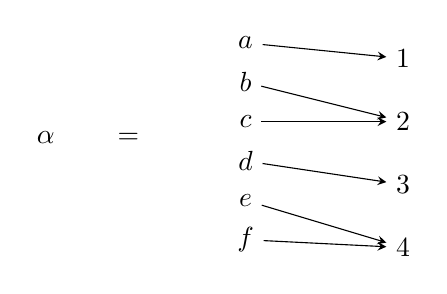
\begin{tikzpicture}[>=stealth, node distance=2cm, baseline={(current bounding box.center)}]
                \node (label) at (0,2.8) {\( \alpha \qquad = \)};

                \node (a) at (2,4) {$a$};
                \node (b) at (2,3.5) {$b$};
                \node (c) at (2,3) {$c$};
                \node (d) at (2,2.5) {$d$};
                \node (e) at (2, 2) {$e$};
                \node (f) at (2,1.5) {$f$};

                \node (1) at (4,3.8) {$1$};
                \node (2) at (4,3) {$2$};
                \node (3) at (4,2.2) {$3$};
                \node (4) at (4,1.4) {$4$};

                \draw[->] (a) -- (1);
                \draw[->] (b) -- (2);
                \draw[->] (c) -- (2);
                \draw[->] (d) -- (3);
                \draw[->] (e) -- (4);
                \draw[->] (f) -- (4);
            \end{tikzpicture}
        \end{center}
        \begin{align*}
            & \implies \Big(\big(e, 4\big) \in \alpha\Big) \wedge \Big(\big(f, \; 4\big) \in \alpha\Big) \\ 
            & \implies \exists x_1 \exists x_2 \exists y \; \Big( \big(x_1, y\big) \in \alpha \Big) \wedge
                                                   \Big( \big(x_2, y\big) \in \alpha \Big) \wedge
                                                   \Big( x_1 \neq x_2 \Big) \\
            & \implies \exists x_1 \exists x_2 \exists y \; \Big( \big(x_1, y\big) \in \alpha \Big) \wedge
                                                   \Big( \big(x_2, y\big) \in \alpha \Big) \wedge
                                                   \neg\Big( x_1 = x_2 \Big) \\
            & \implies \exists x_1 \exists x_2 \exists y \; \Big( \big(x_1, y\big) \in \alpha \wedge
                                                   \big(x_2, y\big) \in \alpha \Big) \wedge
                                                   \neg\Big( x_1 = x_2 \Big) \\
            & \implies \exists x_1 \exists x_2 \exists y \; \neg\Big( \big(x_1, y\big) \in \alpha \wedge
                                                   \big(x_2, y\big) \in \alpha \Big) \lor
                                                   \Big( x_1 = x_2 \Big) \\
            & \implies \exists x_1 \exists x_2 \exists y \; \Big( \big(x_1, y\big) \in \alpha \wedge
                                                   \big(x_2, y\big) \in \alpha \Big) \implies
                                                   \Big( x_1 = x_2 \Big) \\
            & \implies \neg\forall x_1 \forall x_2 \forall y \; \Big( \big(x_1, y\big) \in \alpha \wedge
                                                   \big(x_2, y\big) \in \alpha \Big) \implies
                                                   \Big( x_1 = x_2 \Big) \\
            & \implies \neg\Big( \alpha : D_{\alpha} \rightarrowtail R_{\alpha} \Big)
              \implies \text{ \(\alpha\) is not a one-to-one function.}
        \end{align*}

        \subsection{Function \(\beta\) }
        \vspace{8pt}
        \begin{center}
            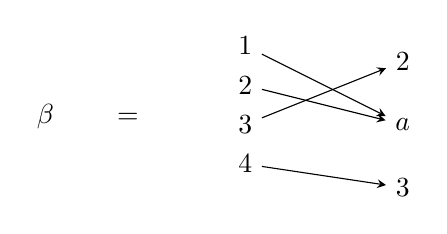
\begin{tikzpicture}[>=stealth, node distance=2cm, baseline={(current bounding box.center)}]
                \node (label) at (0, 3.1) {\( \beta \qquad = \)};

                \node (1) at (2,4) {$1$};
                \node (2D) at (2,3.5) {$2$};
                \node (3D) at (2,3) {$3$};
                \node (4) at (2,2.5) {$4$};

                \node (2R) at (4,3.8) {$2$};
                \node (a) at (4,3) {$a$};
                \node (3R) at (4,2.2) {$3$};

                \draw[->] (1) -- (a);
                \draw[->] (2D) -- (a);
                \draw[->] (3D) -- (2R);
                \draw[->] (4) -- (3R);
            \end{tikzpicture}
        \end{center}
        \begin{align*}
            & \implies \Big(\big(1, a\big) \in \beta\Big) \wedge \Big(\big(2,a\big) \in \beta\Big) \\ 
            & \implies \exists x_1 \exists x_2 \exists y \; \Big( \big(x_1, y\big) \in \beta \Big) \wedge
                                                   \Big( \big(x_2, y\big) \in \beta \Big) \wedge
                                                   \Big( x_1 \neq x_2 \Big) \\
            & \implies \exists x_1 \exists x_2 \exists y \; \Big( \big(x_1, y\big) \in \beta \Big) \wedge
                                                   \Big( \big(x_2, y\big) \in \beta \Big) \wedge
                                                   \neg\Big( x_1 = x_2 \Big) \\
            & \implies \exists x_1 \exists x_2 \exists y \; \Big( \big(x_1, y\big) \in \beta \wedge
                                                   \big(x_2, y\big) \in \beta \Big) \wedge
                                                   \neg\Big( x_1 = x_2 \Big) \\
            & \implies \exists x_1 \exists x_2 \exists y \; \neg\Big( \big(x_1, y\big) \in \beta \wedge
                                                   \big(x_2, y\big) \in \beta \Big) \lor
                                                   \Big( x_1 = x_2 \Big) \\
            & \implies \exists x_1 \exists x_2 \exists y \; \Big( \big(x_1, y\big) \in \beta \wedge
                                                   \big(x_2, y\big) \in \beta \Big) \implies
                                                   \Big( x_1 = x_2 \Big) \\
            & \implies \neg\forall x_1 \forall x_2 \forall y \; \Big( \big(x_1, y\big) \in \beta \wedge
                                                   \big(x_2, y\big) \in \beta \Big) \implies
                                                   \Big( x_1 = x_2 \Big) \\
            & \implies \neg\Big( \beta : D_{\beta} \rightarrowtail R_{\beta} \Big)
              \implies \text{ \(\beta\) is not a one-to-one function.}
        \end{align*}

        \subsection{Relation \(f\) }
        \begin{center}
            \includegraphics[width=0.3\textwidth]{relation_f.png}
        \end{center}
        \begin{align*}
            & \implies \Big(\big(2, 4\big) \in f\Big) \wedge \Big(\big(4, 4\big) \in f\Big) \\ 
            & \implies \exists x \exists y_1 \exists y_2 \; \Big( \big(x, y_1\big) \in f \Big) \wedge
                                                   \Big( \big(x, y_2\big) \in f \Big) \wedge
                                                   \Big( y_1 \neq y_2 \Big) \\
            & \implies \exists x \exists y_1 \exists y_2 \; \Big( \big(x, y_1\big) \in f \Big) \wedge
                                                   \Big( \big(x, y_2\big) \in f \Big) \wedge
                                                   \neg\Big( y_1 = y_2 \Big) \\
            & \implies \exists x \exists y_1 \exists y_2 \; \Big( \big(x, y_1\big) \in f \wedge
                                                   \big(x, y_2\big) \in f \Big) \wedge
                                                   \neg\Big( y_1 = y_2 \Big) \\
            & \implies \exists x \exists y_1 \exists y_2 \; \neg\Big( \big(x, y_1\big) \in f \wedge
                                                   \big(x, y_2\big) \in f \Big) \lor
                                                   \Big( y_1 = y_2 \Big) \\
            & \implies \exists x \exists y_1 \exists y_2 \; \Big( \big(x, y_1\big) \in f \wedge
                                                   \big(x, y_2\big) \in f \Big) \implies
                                                   \Big( y_1 = y_2 \Big) \\
            & \implies \neg\forall x \forall y_1 \forall y_2 \; \Big( \big(x, y_1\big) \in f \wedge
                                                   \big(x, y_2\big) \in f \Big) \implies
                                                   \Big( y_1 = y_2 \Big) \\
            & \implies \neg\Big( f : D_{f} \to R_{f} \Big)
              \implies \text{ \(f\) is not a one-to-one function.}
        \end{align*}

        \subsection{Relation \(f+g\) }
        \begin{center}
            \includegraphics[width=0.3\textwidth]{relation_f+g.png}
        \end{center}
        \begin{align*}
            & \implies \Big(\big(3, 4\big) \in f+g\Big) \wedge \Big(\big(4, 4\big) \in f+g\Big) \\ 
            & \implies \exists x \exists y_1 \exists y_2 \; \Big( \big(x, y_1\big) \in f+g \Big) \wedge
                                                   \Big( \big(x, y_2\big) \in f+g \Big) \wedge
                                                   \Big( y_1 \neq y_2 \Big) \\
            & \implies \exists x \exists y_1 \exists y_2 \; \Big( \big(x, y_1\big) \in f+g \Big) \wedge
                                                   \Big( \big(x, y_2\big) \in f+g \Big) \wedge
                                                   \neg\Big( y_1 = y_2 \Big) \\
            & \implies \exists x \exists y_1 \exists y_2 \; \Big( \big(x, y_1\big) \in f+g \wedge
                                                   \big(x, y_2\big) \in f+g \Big) \wedge
                                                   \neg\Big( y_1 = y_2 \Big) \\
            & \implies \exists x \exists y_1 \exists y_2 \; \neg\Big( \big(x, y_1\big) \in f+g \wedge
                                                   \big(x, y_2\big) \in f+g \Big) \lor
                                                   \Big( y_1 = y_2 \Big) \\
            & \implies \exists x \exists y_1 \exists y_2 \; \Big( \big(x, y_1\big) \in f+g \wedge
                                                   \big(x, y_2\big) \in f+g \Big) \implies
                                                   \Big( y_1 = y_2 \Big) \\
            & \implies \neg\forall x \forall y_1 \forall y_2 \; \Big( \big(x, y_1\big) \in f+g \wedge
                                                   \big(x, y_2\big) \in f+g \Big) \implies
                                                   \Big( y_1 = y_2 \Big) \\
            & \implies \neg\Big( f : D_{f+g} \to R_{f+g} \Big)
              \implies \text{ \(f+g\) is not a one-to-one function.}
        \end{align*}

    







\end{document}

